\subsubsection{Análisis para $R_{comp_{4}}$ en modo corriente, $I_{out} = 200 \si[per-mode=symbol]{\milli\ampere}$, $R_{L} = 0 \si[per-mode=symbol]{\ohm}$}

Se puede ver en la figura~\figref{fig:fig_power_supply_RCOMP4_LOOP_Modo4} como con el valor de $C_{comp_{4}} = 1 \si[per-mode=symbol]{\kilo\ohm}$ se logra unos márgenes de fase y ganancia aceptables, valores menores podrían ser mas convenientes en este caso, además seguir aumentando el valor de $C_{comp_{4}}$, no cambian mucho el ancho de banda de la respuesta en frecuencia, como se puede ver en la figura~\figref{fig:fig_power_supply_RCOMP4_RF_Modo4}. A nivel de respuesta dinámica el comportamiento es inverso respecto al tiempo de crecimiento, ver figura~\figref{fig:fig_power_supply_RCOMP4_STEP_500_Modo4}, figura~\figref{fig:fig_power_supply_RCOMP4_STEP_1k_Modo4} y figura~\figref{fig:fig_power_supply_RCOMP4_STEP_2k_Modo4}.

\vfill


%% CCOMP4 MODO 4.

\clearpage

\begin{figure}[H] %htb
\begin{center}
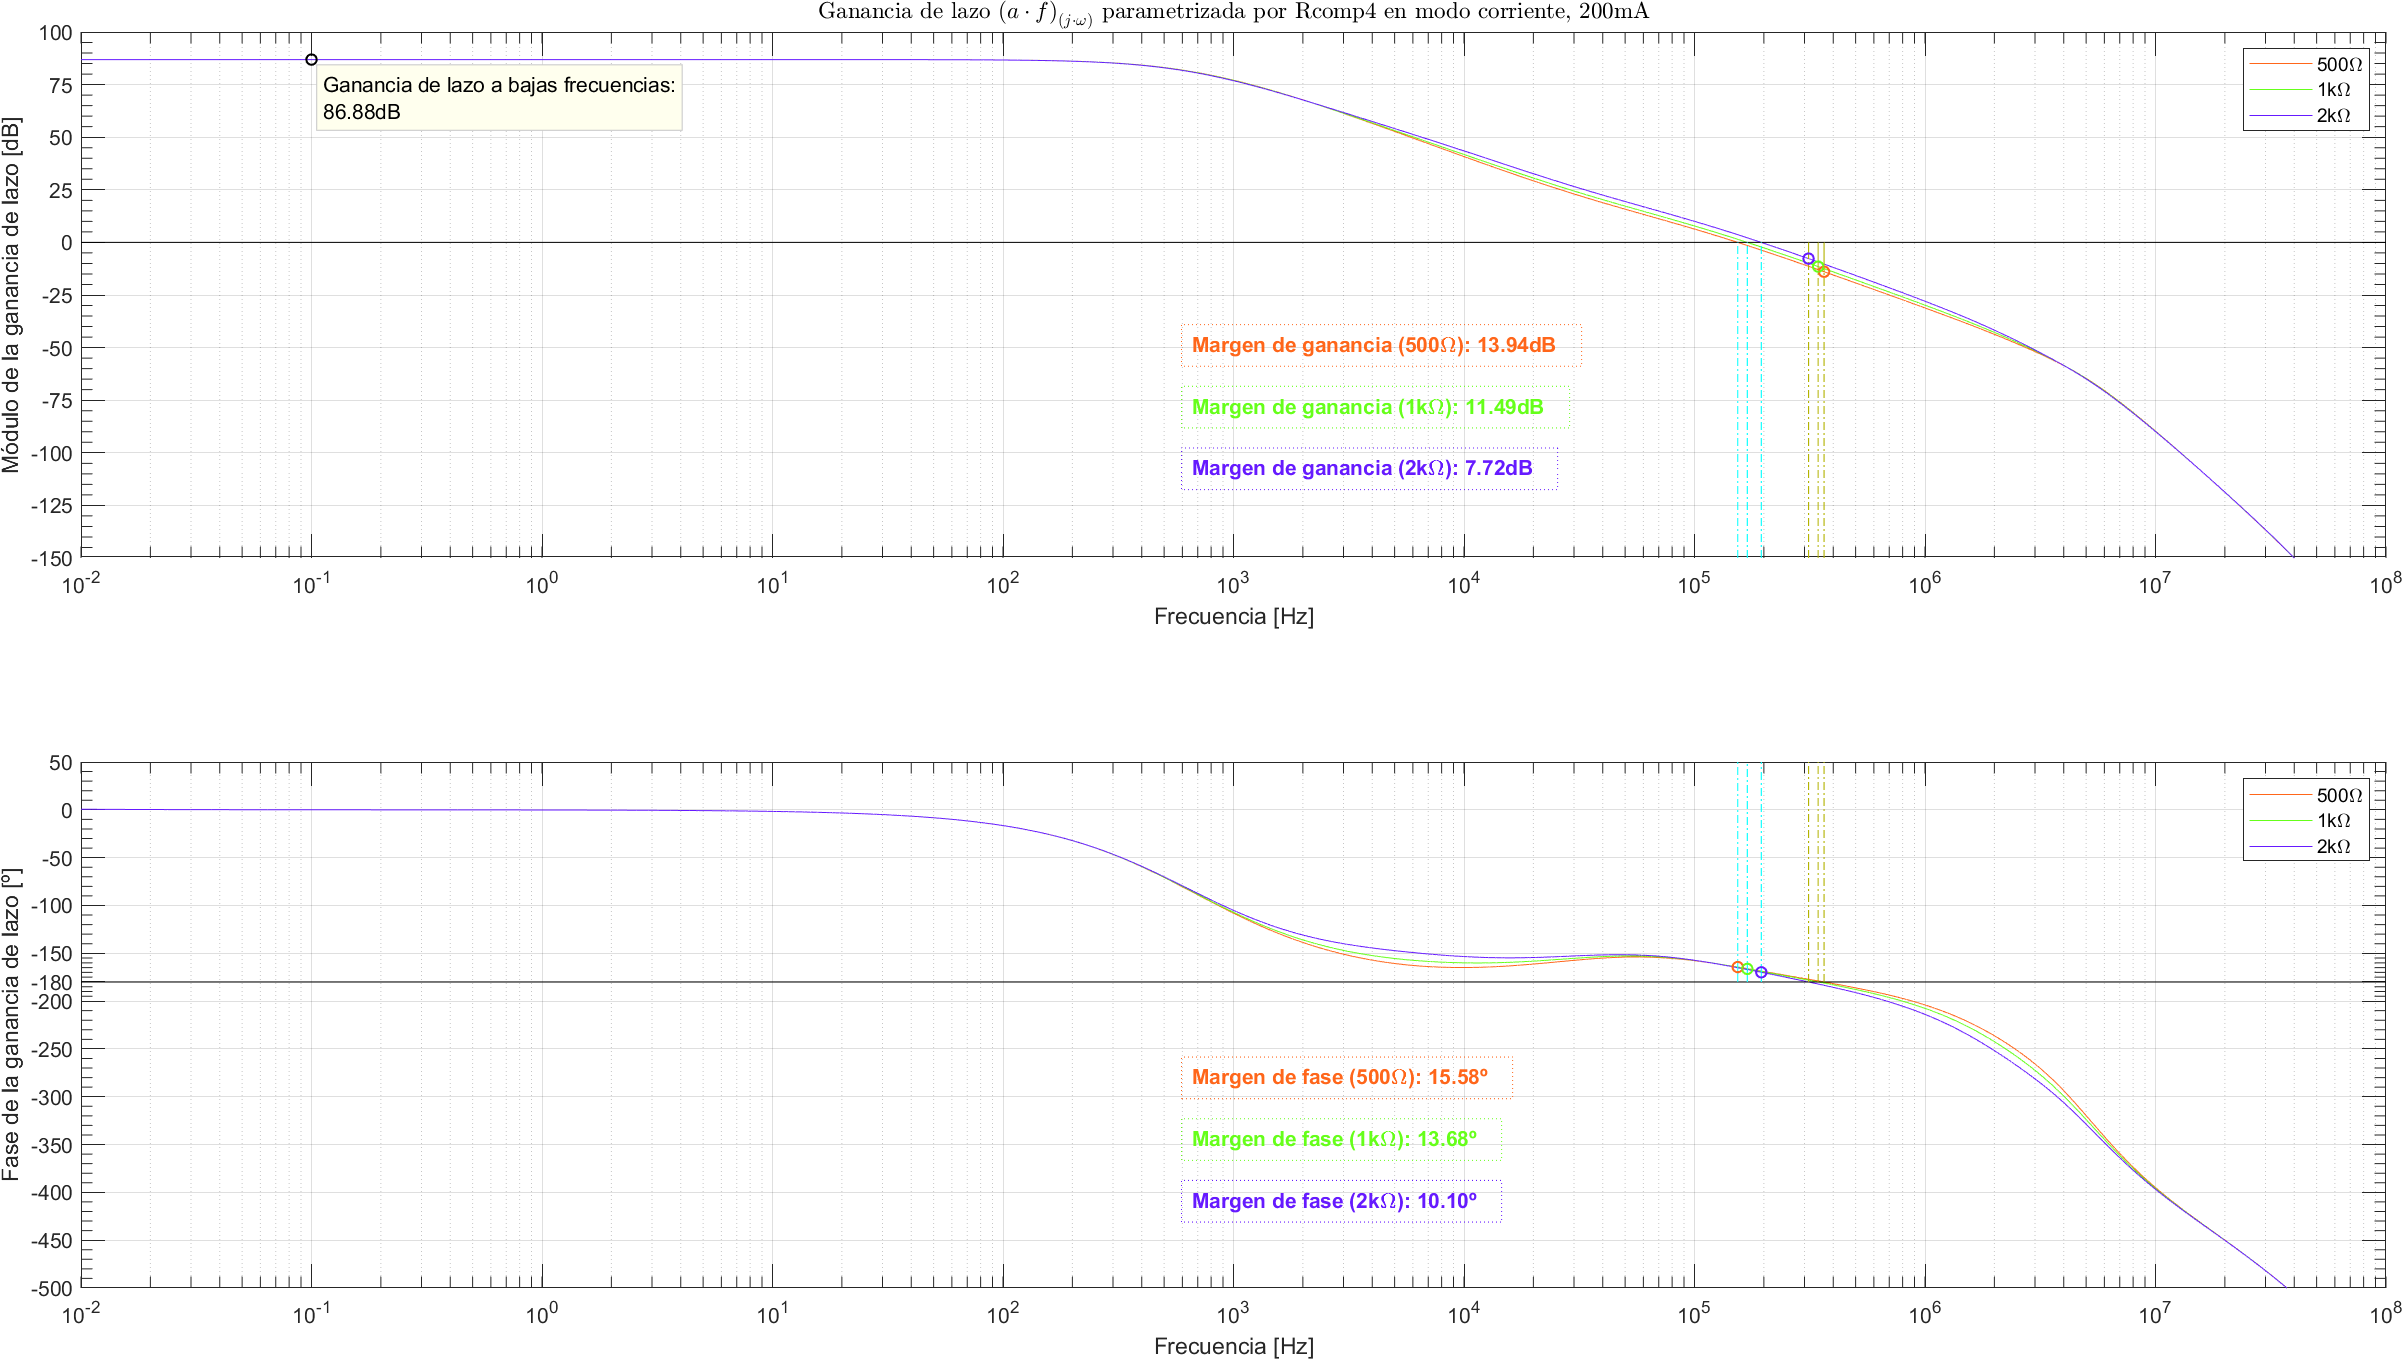
\includegraphics[width=1.1 \textwidth, angle=90]{./img/plots/loop/power_supply_RCOMP4_LOOP_Modo4.png}
\caption{\label{fig:fig_power_supply_RCOMP4_LOOP_Modo4}\footnotesize{Ganancia de lazo en modo corriente, $I_{out} = 200 \si[per-mode=symbol]{\milli\ampere}$, en función de la frecuencia parametrizada por $R_{comp_{4}}$.}}
\end{center}
\end{figure}


\clearpage

\begin{figure}[H] %htb
\begin{center}
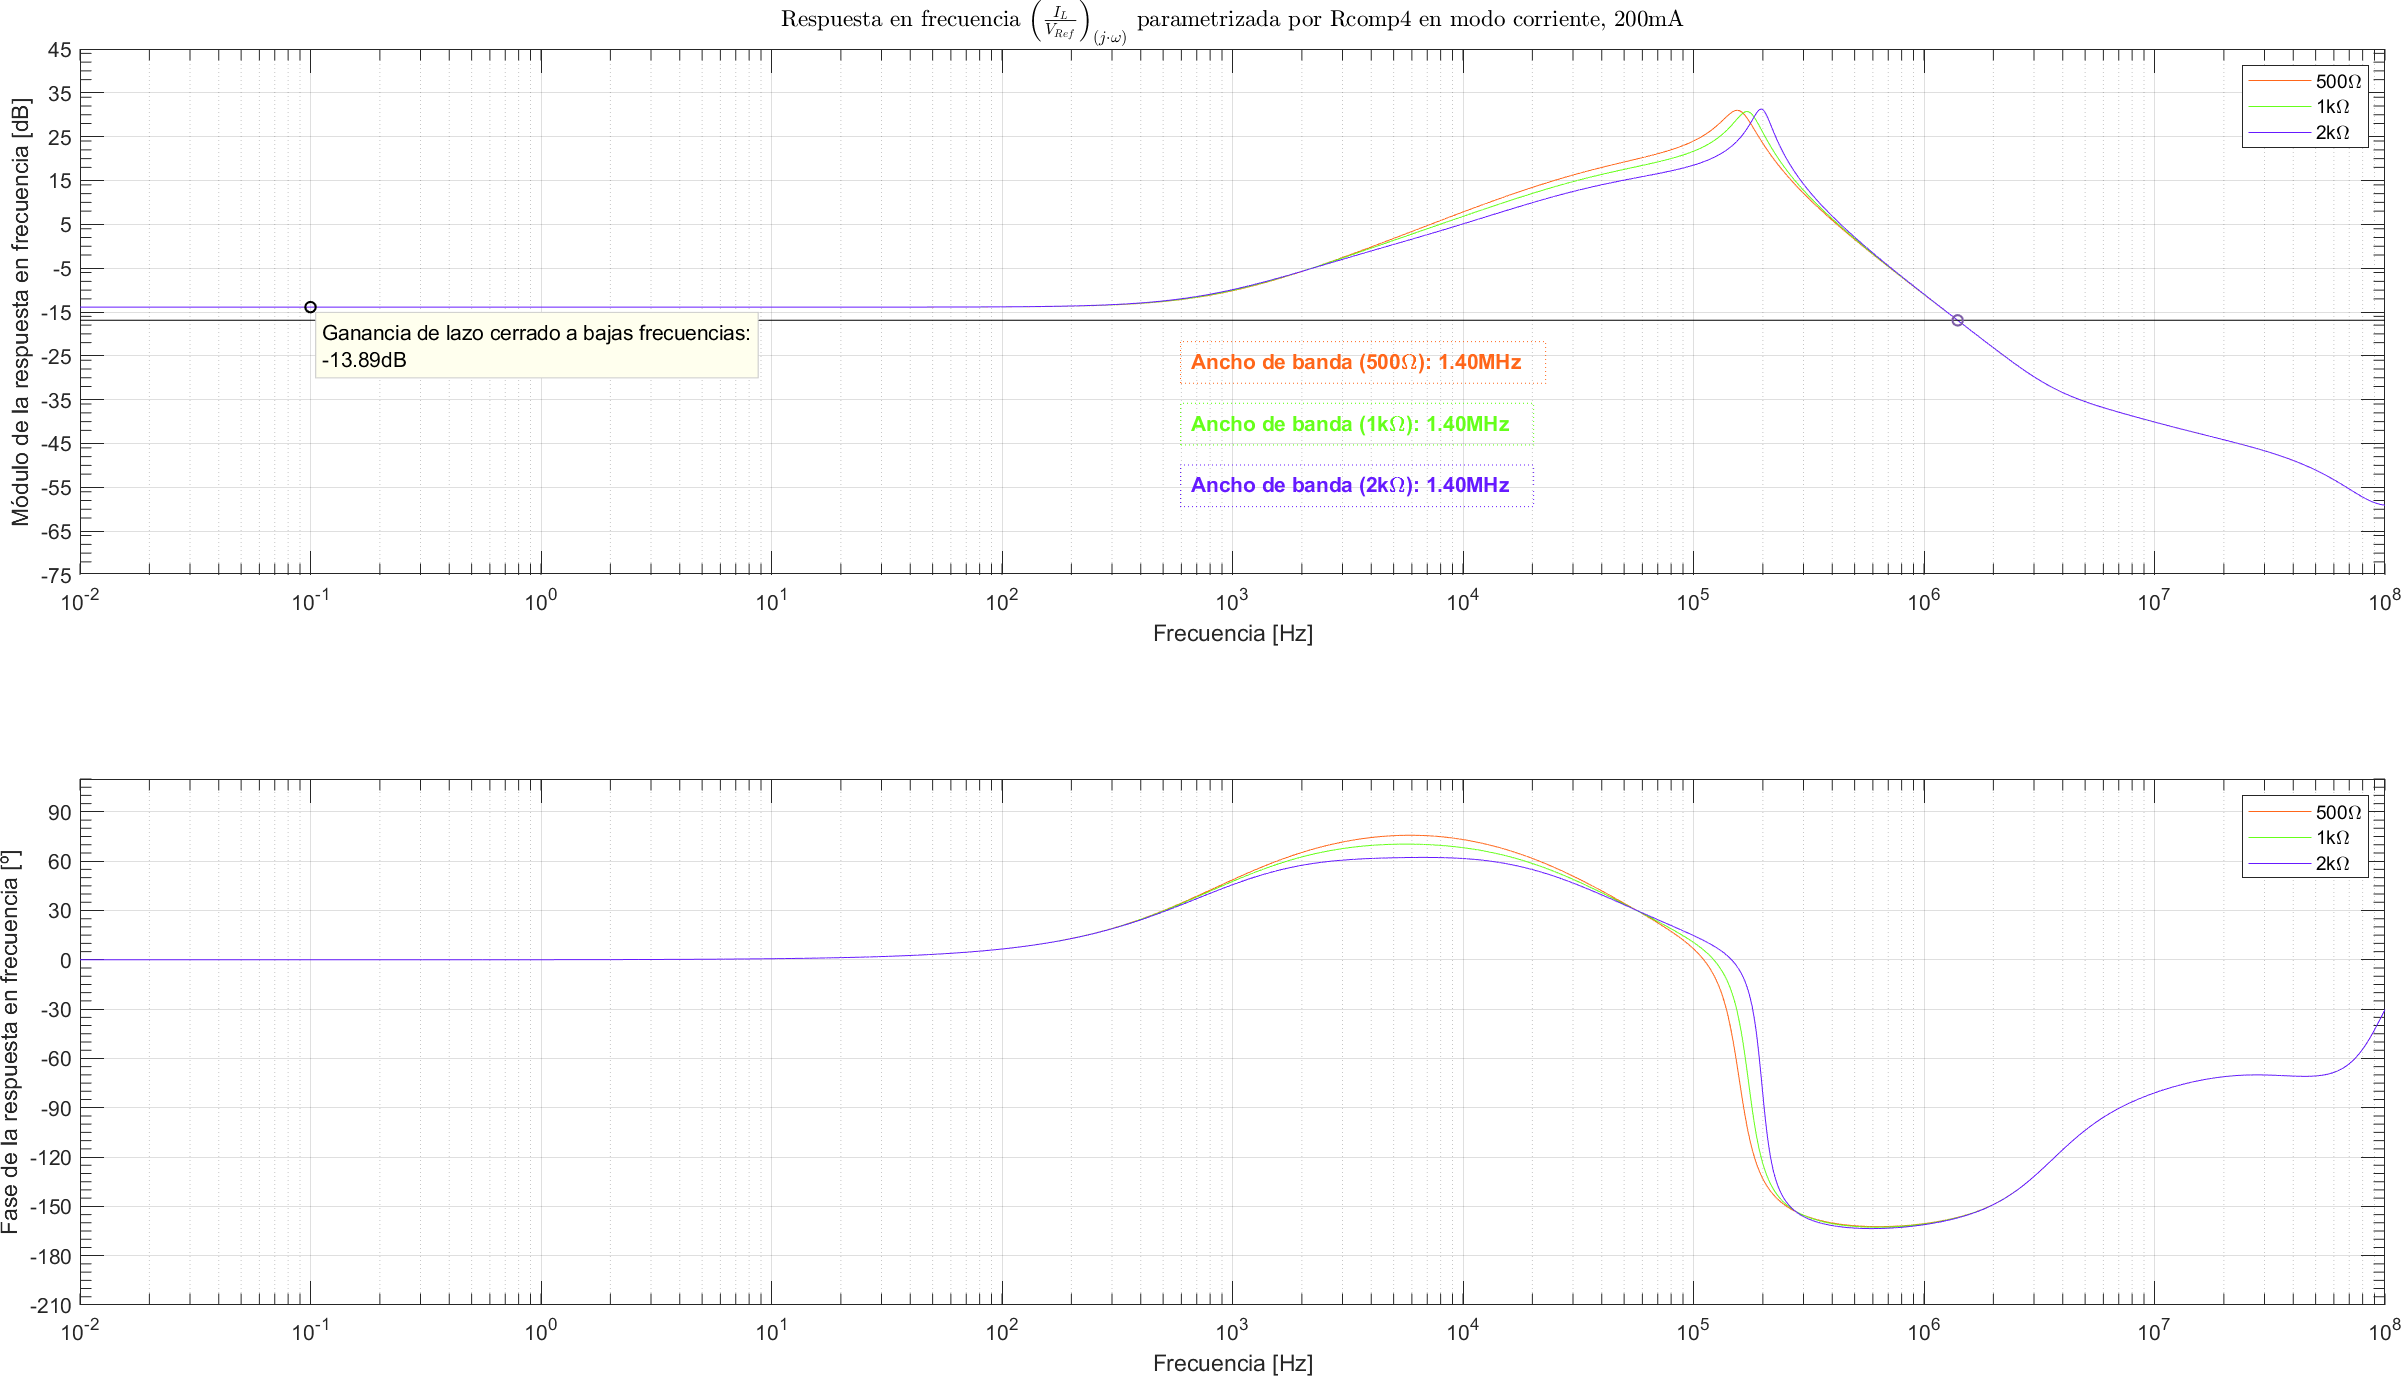
\includegraphics[width=1.1 \textwidth, angle=90]{./img/plots/rf/power_supply_RCOMP4_RF_Modo4.png}
\caption{\label{fig:fig_power_supply_RCOMP4_RF_Modo4}\footnotesize{Respuesta en frecuencia en modo corriente, $I_{out} = 200 \si[per-mode=symbol]{\milli\ampere}$, en función de la frecuencia parametrizada por $R_{comp_{4}}$.}}
\end{center}
\end{figure}

\clearpage

\begin{figure}[H] %htb
\begin{center}
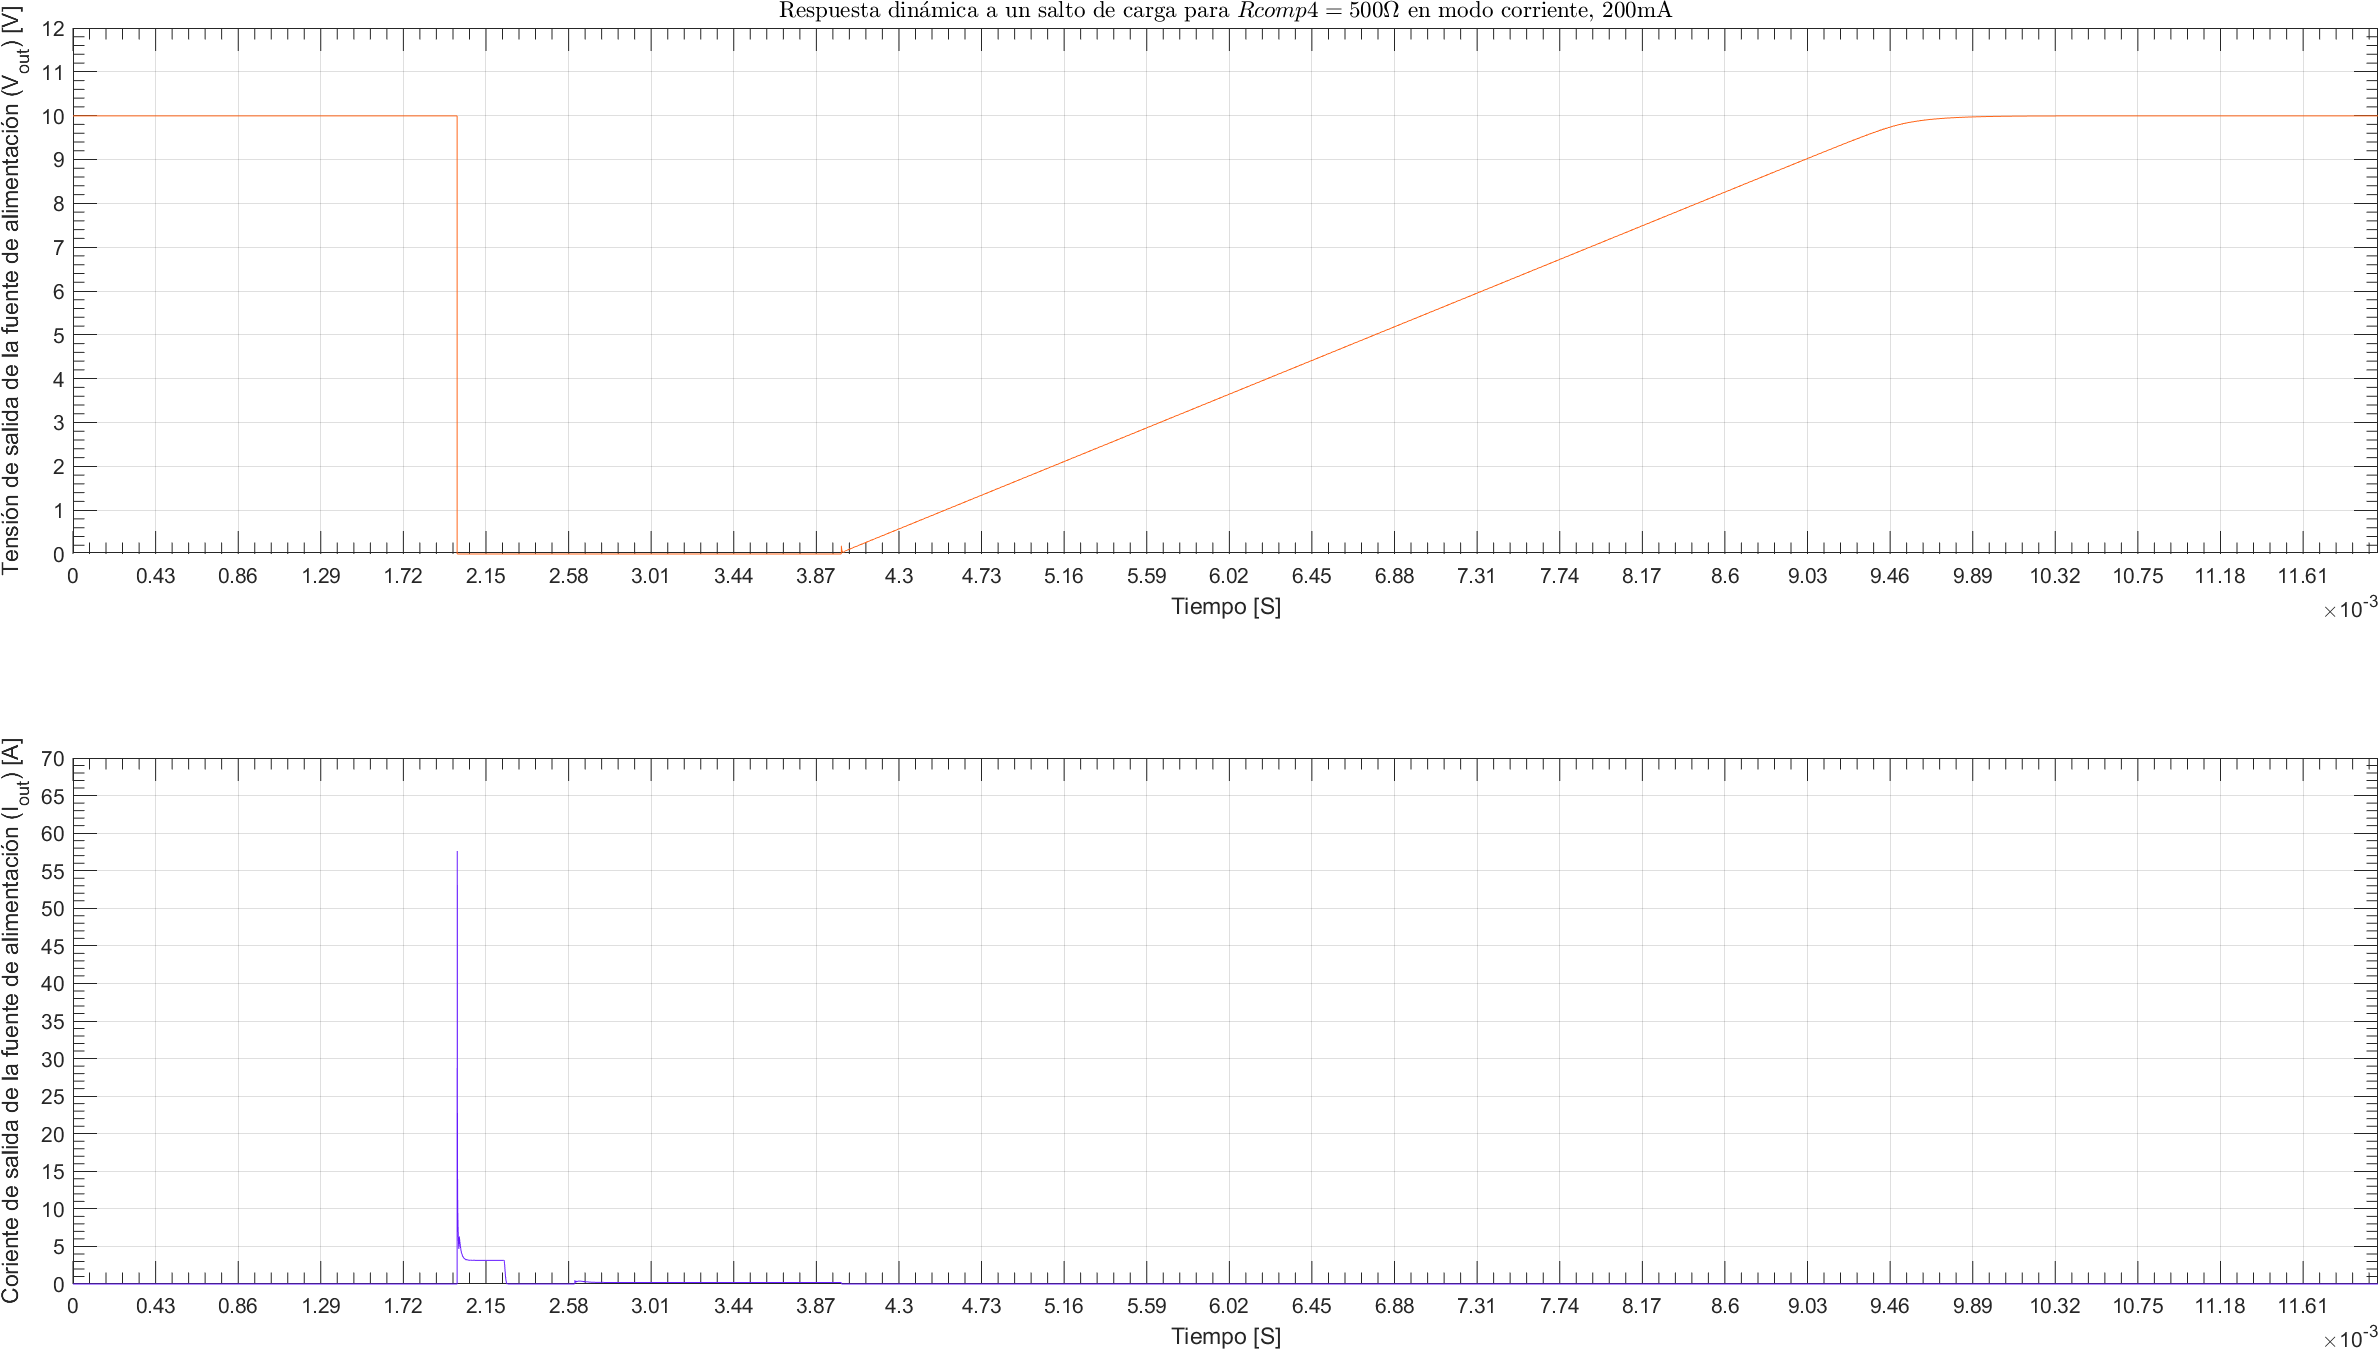
\includegraphics[width=1.1 \textwidth, angle=90]{./img/plots/dynamic/power_supply_RCOMP4_500_STEP_Modo4.png}
\caption{\label{fig:fig_power_supply_RCOMP4_STEP_500_Modo4}\footnotesize{Respuesta dinámica en modo corriente, $I_{out} = 200 \si[per-mode=symbol]{\milli\ampere}$, para $R_{comp_{4}} = 500 \si[per-mode=symbol]{\ohm} $.}}
\end{center}
\end{figure}

\clearpage

\begin{figure}[H] %htb
\begin{center}
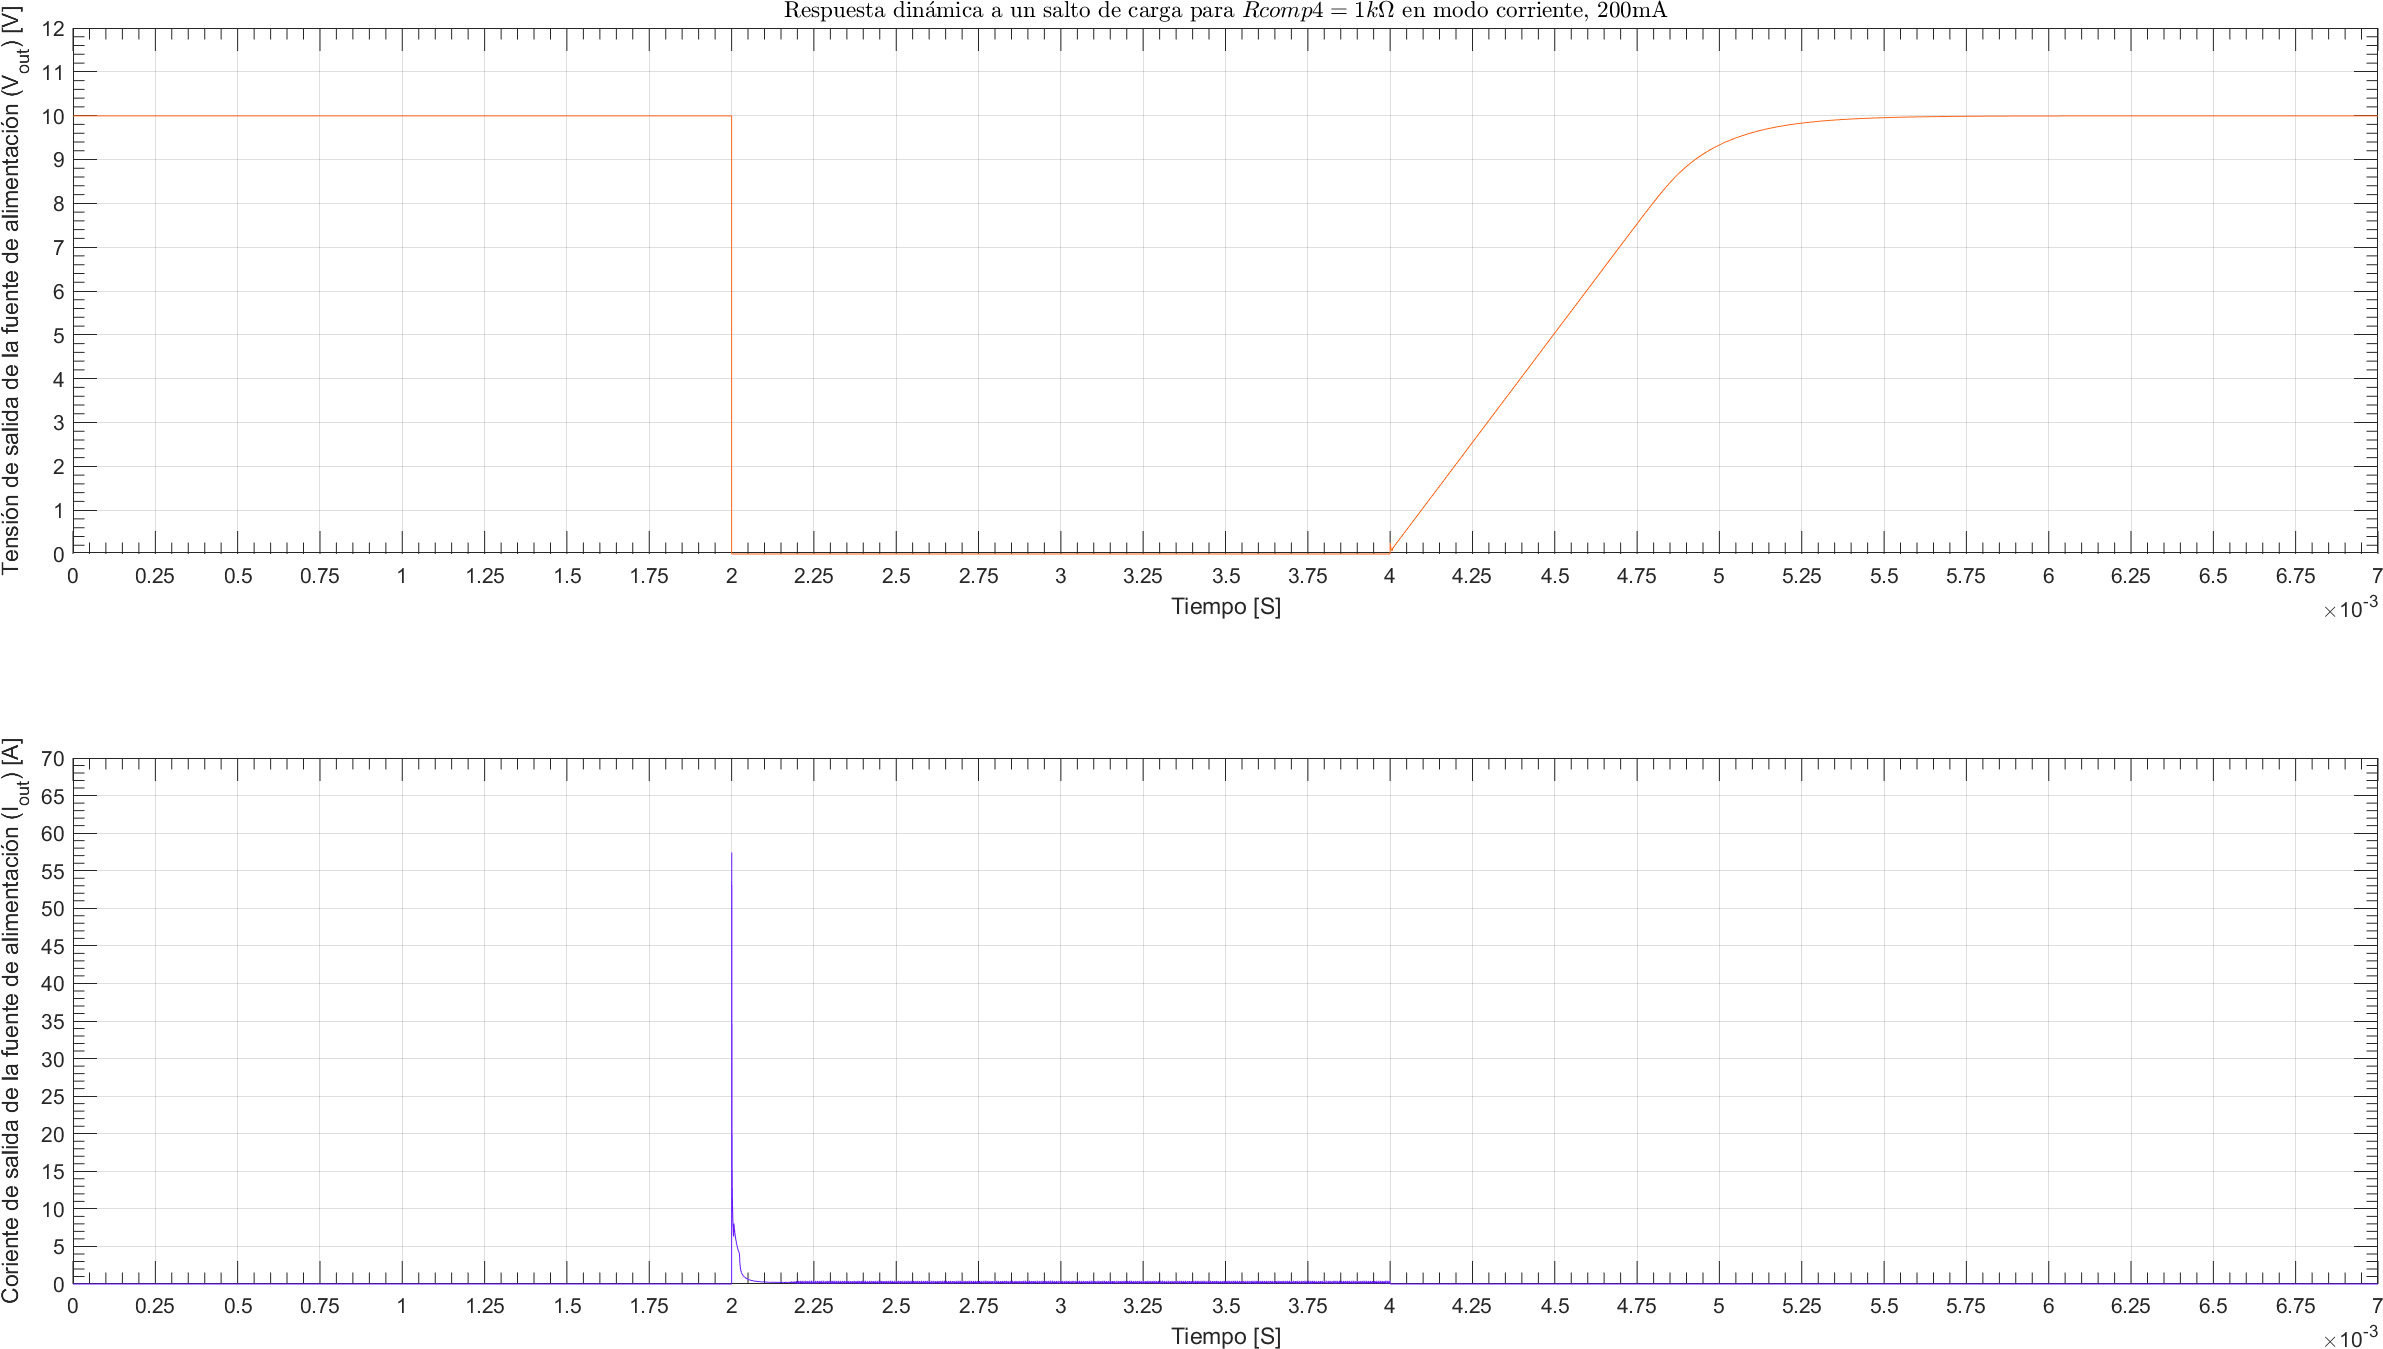
\includegraphics[width=1.1 \textwidth, angle=90]{./img/plots/dynamic/power_supply_RCOMP4_1k_STEP_Modo4.png}
\caption{\label{fig:fig_power_supply_RCOMP4_STEP_1k_Modo4}\footnotesize{Respuesta dinámica en modo corriente, $I_{out} = 200 \si[per-mode=symbol]{\milli\ampere}$, para $R_{comp_{4}} = 1 \si[per-mode=symbol]{\kilo\ohm} $.}}
\end{center}
\end{figure}

\clearpage

\begin{figure}[H] %htb
\begin{center}
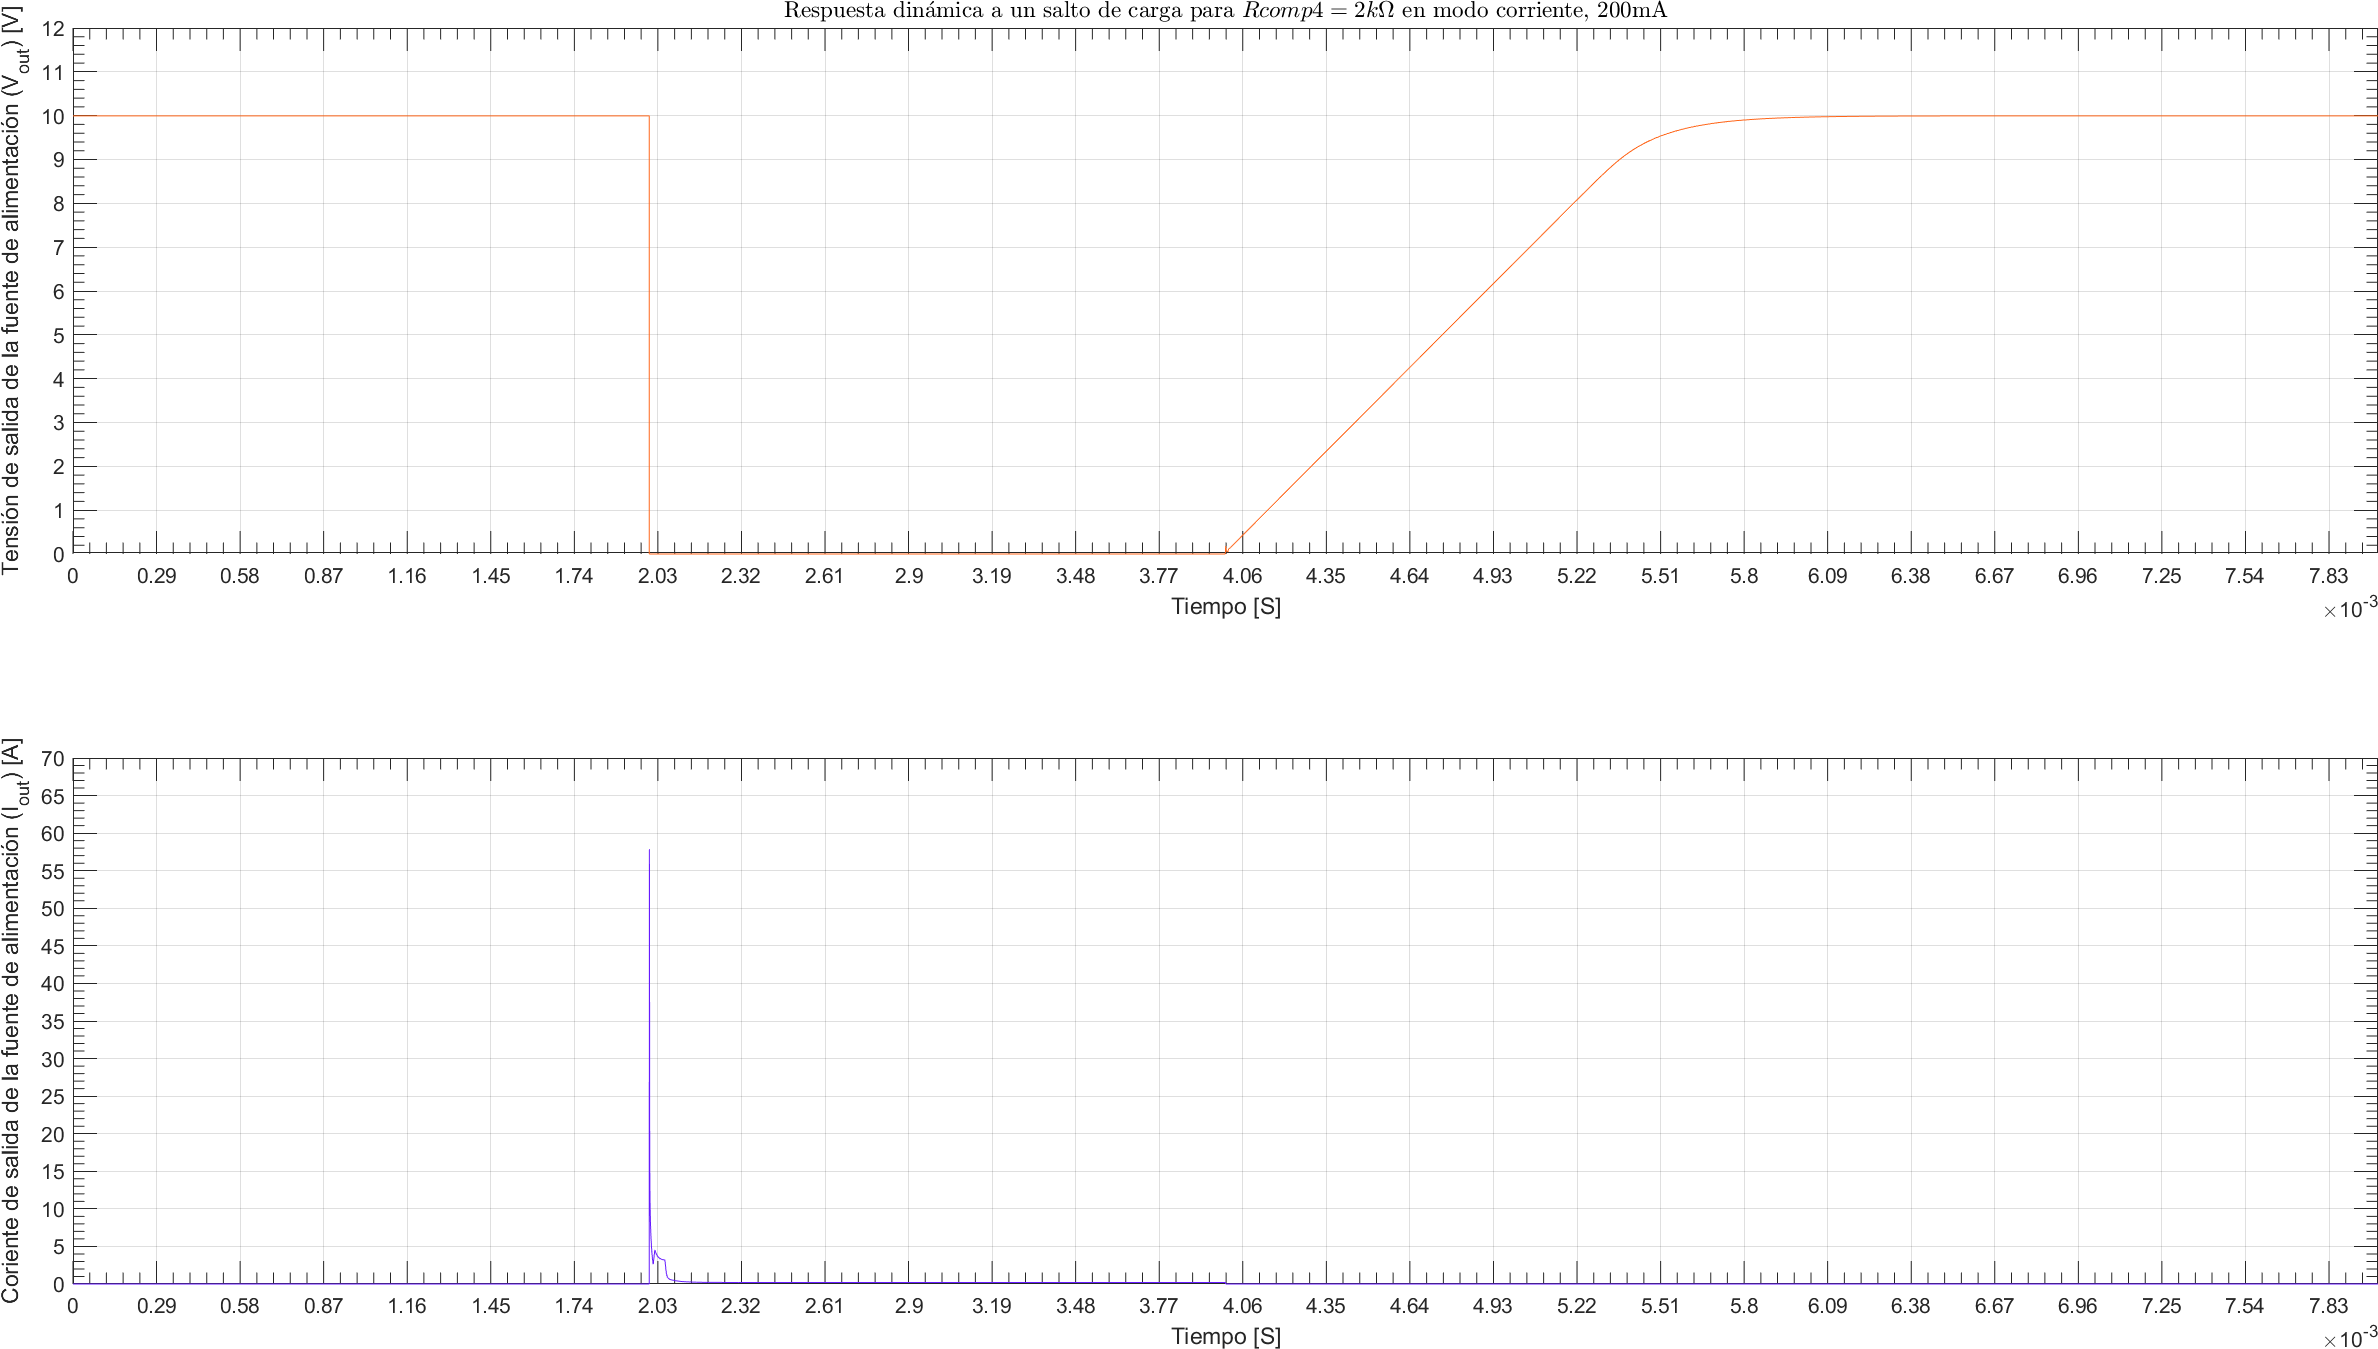
\includegraphics[width=1.1 \textwidth, angle=90]{./img/plots/dynamic/power_supply_RCOMP4_2k_STEP_Modo4.png}
\caption{\label{fig:fig_power_supply_RCOMP4_STEP_2k_Modo4}\footnotesize{Respuesta dinámica en modo corriente, $I_{out} = 200 \si[per-mode=symbol]{\milli\ampere}$, para $R_{comp_{4}} = 2 \si[per-mode=symbol]{\kilo\ohm} $.}}
\end{center}
\end{figure}

\clearpage




